\documentclass[article]{aaltoseries}
\usepackage[utf8]{inputenc}
\usepackage{hyperref}
\usepackage{cleveref}
\usepackage{multirow} % Multi row cells in table
\usepackage{pdflscape}
\usepackage{array, ltablex} 

\usepackage{xargs}
\usepackage[textsize=footnotesize,obeyFinal]{todonotes}

\newcommand{\todonotes}[2]{\todo[inline,color={#1}]{#2}}
\newcommand{\note}[1]{\todonotes{green!20!white}{#1}}
\newcommand{\warning}[1]{\todonotes{orange!20!white}{#1}}
\newcommand{\question}[1]{\todonotes{red!20!white}{#1}}
\newcommand{\blocking}[1]{\todonotes{red!40!white}{#1}}
\newcommand{\grammar}[1]{\todonotes{blue!20!white}{#1}}

\renewcommand{\autoref}[1]{\href{#1}{\Cref{#1}}}

\begin{document}

% Bibtex: use howpublished = {\url{#1}},
 
%=========================================================

\title{A Review on the Status of Serverless Computing at the Edge of Public Cloud Platforms}

\author{
Adriaan Knapen% Your first and last name: do _not_ add your student number
    \\\textnormal{
        \texttt{
            \href{mailto:adriaan.knapen@aalto.fi}{adriaan.knapen@aalto.fi}% Your Aalto e-mail address
        }
    }
}
\affiliation{\textbf{Tutor}: Gopika Premsankar} % First and last name of your tutor
\maketitle
%==========================================================

\begin{abstract}
Public cloud providers now provide serverless computing on edge devices to process an ever increasing amount of data generated by internet-of-things (IoT) devices. 
Employing edge computing has been shown to reduce the high latency, bandwidth usage and costs involved with using cloud solutions. 
Public cloud solution providers, including Amazon AWS, Microsoft Azure and Google Cloud, have been developing edge solutions to complement their cloud offerings.
Such providers have been looking into employing the serverless paradigm on the edge, such that the serverless functions currently deployed on the public cloud can be transferred to edge nodes.
This paper starts with a discussion on the advantages and challenges of employing serverless at the edge. 
We then describe the main features of the edge solutions offered by the following cloud providers: Amazon, Microsoft, Google and IBM.
% Next, we propose a method, supported by experimental results, which offers lower latency for tasks with widely varying computational costs by simultaneously executing them on both the edge and cloud.
% Finally we conclude with our experiences deploying the serverless edge solutions on AWS Greengrass and Microsoft Azure IoT Edge.

\vspace{3mm}
\noindent KEYWORDS: Edge Computing, Function-as-a-Service, FaaS, Serverless, Cloud Computing, Internet of Things, IoT, AWS Greengras, Microsoft Azure IoT Edge

\end{abstract}

%============================================================
% Should the topic be kept distinct from fog computing?

% Review other framework comparison papers

% Query on serverless edge computing platforms

% \note{This is a side note}
% \warning{This is a warning, mainly used for to-dos}
% \question{This is a non-blocking question}
% \blocking{This is a blocking question}
% \grammar{This is a grammar related question}

\section{Introduction} 
The emergence of public cloud computing solutions has been an important factor in the growing success of the Internet of Things (IoT). %~\cite{shi_promise_2016}.
This is mainly because these cloud solutions allows vast amounts of data to be processed efficiently, something which is not attainable when processing the data directly on the IoT devices~\cite{shi_promise_2016}.
Although IoT has greatly benefited from cloud solutions, it also introduces various limitations.
Using the cloud as the data processing backend for IoT introduces several problems, including high latency and bandwidth constraints~\cite{shi_edge_2016}.
For instance, \emph{high latency} is problematic when making driving decisions for autonomous cars~\cite{shi_promise_2016}, whereas the \emph{bandwidth constraints} are crucial when running facial recognition software on video footage from a large number of cameras~\cite{taleb_multi-access_2017}.
One of the methods proposed to address this issue is \emph{edge computing}~\cite{shi_edge_2016}.
% Edge computing places computation resources at the edge of the network, that is, close to the end user and within the same local area network.
In the context of edge computing do we consider all computing and networking resources as \emph{edge devices} if they are on the path from cloud data centers to the data source.
Edge computing refers to the technologies enabling edge devices to take on part of the tasks of either the cloud or end-devices~\cite{shi_edge_2016}. 
In this context, we consider \emph{edge devices}, also known as \emph{edge nodes}, to consist of any computing and networking resource on the path from the end-device to the cloud.
Hence edge devices cover a wide variety of devices, ranging from those with low computation power, such as smartphones, to compute intensive specialized micro-datacenters~\cite{shi_promise_2016}.

% Make the link between this section and the topic serverless edge computing more clear.
% Maybe put it back, since the teacher for Academic Communication likes it.

% However, often it is not sufficient to merely employ edge devices, because there is no central node which has a global view of all employed edge nodes.
% The necessity of a globally accessible system for all edge devices often originates from the demand for global data mining~\cite{bonomi_fog_2012}.
% One method of addressing this necessity is using cloud solutions.
% Combining edge and cloud computing has shown to be advantageous.
% Employing such combination of edge and cloud has been shown to increase the execution speed and decrease in energy consumption by a factor of 20~\cite{chun_clonecloud:_2011} compared to merely using cloud solutions.

Previous research has proposed combining edge computing with a serverless cloud solution~\cite{de_paoli_empowering_2017, glikson_deviceless_2017, nastic_serverless_2017}.
The serverless paradigm, also known as Function-as-a-Service (FaaS), offers a platform which executes user-defined functions on automatically managed distributed platforms~\cite{nastic_serverless_2017}.
Several platforms which support serverless edge computing have emerged, such as AWS Greengrass and Microsoft Azure IoT Edge. % @todo find citation/source
% To our best knowledge, no previous research has conducted an analysis on the enterprise serverless edge computing platforms.
This paper provides an overview of, and feature analysis comparison on, the two different platforms discussed above and a solution combining IBM Cloud Functions with Apache OpenWhisk. % @todo add rationale behind the selection of platforms

The remainder of this paper consists of the following sections.
\autoref{sec:pros-and-cons} discusses the advantages and challenges related to employing a serverless approach on the edge.
%\autoref{sec:use-cases} discusses various use cases of adding edge computing to public clouds with a serverless architecture.
% \autoref{sec:feature-selection} presents the features which will be used to compare the different platforms with. % "with" should not be at the end of the sentence.
Then \autoref{sec:overview} introduces the various public cloud platforms. % and their suggested use cases.
\autoref{sec:feature-comparison} compares the platforms based on several features.
% \autoref{sec:experiment} proposes a method, supported by experimental results, on lowering latency for tasks with widely varying computational costs. 
\autoref{sec:discussion-conclusion} concludes this paper with a discussion on the findings and proposes some future areas of research.

%============================================================
\section{Serverless at the Edge}\label{sec:pros-and-cons}
Edge computing has some major advantages over cloud computing, including lower latency, decrease in bandwidth usage and offline operation~\cite{shi_edge_2016}. % find source of offline operation
However the wide variety of the hardware employed as edge devices forces developers to create situation specific solutions, which is a laborious, error-prone and task-specific process~\cite{nastic_serverless_2017}.
This imposes two major disadvantages, first it is harder to re-use previously developed solutions.
Secondly large-scale deployment on a set of heterogeneous resources will be difficult, if not impossible, as a result of the complications arising of deploying the same solution on a wide range of hardware~\cite{nastic_serverless_2017}.

Employing serverless computing at the edge nodes tries to address these issues.
The serverless approach at the edge tries to simplify development by offering a homogeneous development interface, which abstracts deployment specifics away from the developer.
Since the serverless applications do not include deployment specific features this allows easier reuse and deployment of the same solutions on heterogeneous set of hardware~\cite{nastic_serverless_2017}.

De Paoli et al. \cite{de_paoli_empowering_2017} suggests using serverless edge computing for augmented reality (AR) on mobile devices.
They propose a solution to leverage these edge nodes to capture features from images taken by the user's mobile device.
Specifically, the above mentioned use case focuses on helping tourists who are visiting a city by giving relevant information for Points-of-Interest by pointing the camera of their mobile devices at them.
The edge node then augments the received visual using various methods, e.g., by adding relevant information, modifying the content of the image or adding virtual elements. 
Using edge computing to address this issue is particularly useful, because it offloads the computation-intensive task of feature extraction to another device, saving battery on the phone, while keeping the latency lower than what would have been possible when using the cloud.
Thus optimizing for the experience of the end-user.
% Although using a cloud solution instead of the proposed edge solution would solve the resource constraint problem, however does the cloud induce some negative side effects degrading the user experience, as a result of high latency, possible unstable connections and vast amounts of bandwidth usage.
In addition, feature identification on images does not induce statefulness between different computations, since previous results of mapped features are not used in later computation invocations, which makes this a suitable application for serverless edge computing~\cite{de_paoli_empowering_2017}.

Several challenges arise when employing serverless at the edge~\cite{glikson_deviceless_2017, nastic_serverless_2017}:
\begin{description}
    \item[Security] 
    Serverless platforms in the cloud are protected by the firewall of the data center.
    Moving the serverless functionality outside of this protected environment exposes these edge devices to new types of attacks. 
    Hence when designing for the security mechanisms of serverless edge devices different protection and isolation mechanisms should be considered.
    \item[Large scale provisioning and management] Devices in an edge environment are highly heterogeneous in hardware and geography. Moreover, they can have intermittent networking connectivity. Thus the management of large scale edge device networks requires more advances provisioning and management tools compared to deployment of cloud solutions.
    \item[Elasticity and resource pooling] The geographical dispersion, varying available resources and limited discoverability of the edge nodes requires different approaches to resource pooling and its optimization than the methods employed on the cloud solutions, e.g., by using a peer-to-peer approach instead of centralized.
    \item[Data management] Synchronizing real-time data changes between several edge devices has been demonstrated as increasingly difficult compared to cloud solutions, which can use a single data storage interface for all its compute nodes.
    Resource constraints on the edge, including bandwidth and storage, often make it impossible to synchronize all data and their changes.
    Instead only a selection of or preprocessed set of the data should be considered for synchronization, which might cause suboptimal results compared to cloud solutions leveraging the complete data set.
\end{description}

%============================================================
\section{Overview of Enterprise Serverless Edge Computing Platforms}\label{sec:overview}
% \note{Should suggested use cases of each platform also be included? As done in \cite{lynn_preliminary_2017}}

\subsection{Amazon Web Services}
Amazon Web Services (AWS) offers AWS Greengrass~\cite{amazon_aws_nodate} as a service to employ the AWS serverless cloud platform AWS Lambda on the edge.
Greengrass introduces the Greengrass Core (GGC) runtime, which can be deployed on low powered devices, such as, a Raspberry Pi, positioned as edge nodes.
These edge nodes allow nearby devices running Amazon FreeRTOS or IoT Device SDK to execute the same functions as they would have done on AWS Lambda on the GGC node instead.
In addition does Greengrass handle the firmware and software updates for the code running on its GGC nodes.
A Greengrass Core node is not required to be continuously connected to the AWS cloud, because the node will still allow execution of AWS Lambda on the locally available data.
The core node automatically synchronize its data with the cloud and retrieve all available updates over the air when the connection is restored~\cite{amazon_aws_nodate}.

AWS offers Lambda@Edge as another solution in an attempt to address latency issues when executing serverless functions in the cloud.
However it does not allow computations to be executed on edge devices.
Instead the service automatically selects the AWS datacenter closest to the end-user when executing AWS Lambda functions~\cite{amazon_customizing_nodate}.

\subsection{Microsoft Azure} % https://docs.microsoft.com/en-us/azure/iot-edge/about-iot-edge
Microsoft offers Azure IoT Edge~\cite{microsoft_iot_2018} as their edge computing platform, which includes supports for serverless at the edge.
Microsoft Azure IoT Edge is targeted to run on hardware ranging from low powered devices, for example, a Raspberry Pi, to the most resourceful devices.
The Azure IoT Edge environment can run on both Windows or Linux based hosts.
This environment uses a container based system, powered by Docker, to process the input data it receives.
It supports routing the output of one docker image to another, creating data processing pipelines with multiple stages.
Microsoft supplies containers of various Azure services, including Azure Functions, allowing the deployment of serverless functionality on the edge devices~\cite{microsoft_what_nodate}.
The use cases suggested by Microsoft cover: machine learning where the models are created in the cloud and pushed to the edge devices, stream analytics and self-implemented functionality running on Azure~Functions containers~\cite{microsoft_creating_nodate}.

\subsection{IBM Cloud}
IBM is the creator of Apache OpenWhisk~\cite{the_apache_software_foundation_apache_nodate}, an open-source serverless framework.
IBM uses a slightly modified version of Apache OpenWhisk in their public cloud IBM Cloud to offer IBM Cloud Functions~\cite{lynn_preliminary_2017}.
Consequently, serverless functions can easily be made to deploy on both platforms.
Apache OpenWhisk can be deployed on-premise~\cite{the_apache_software_foundation_apache_nodate}, which allows to deploy it as a serverless computation platform on the edge.
IBM made no specific efforts to support integration between IBM Cloud and self-hosted edge instances of OpenWhisk.

\subsection{Google Cloud}
Google Cloud IoT Edge~\cite{google_edge_nodate} is a part of Google Cloud and intends to bring Google Cloud IoT Core functionality to edge devices.
The platform is mainly focused on machine learning applications and does not does not specifically support running user-defined serverless functions at the edge.
Therefore the platform is not in scope of this paper.
However, we describe the main features of the Cloud IoT Edge solution.
Cloud IoT Edge allows inference of machine learning models at edge nodes.
These models are trained in the Google Cloud, since the cloud has more computational resources than edge nodes.
The data and machine learning model are locally available at the edge nodes, hence they will still function with an intermittent connection to the Google Cloud. % https://cloud.google.com/iot-edge/
The Google Cloud IoT Edge runs on top of both the Android Things and Linux operating system. % https://cloud.google.com/iot-edge/
There is a strong emphasis on hardware acceleration on the edge nodes, both with \emph{graphical processing units} (GPUs) and \emph{tensor processing units} (TPUs)~\cite{google_cloud_nodate}.
For TPUs, Google offers a specialized solution named Edge TPU\texttrademark, which leverages the power of their self-designed purpose-build \emph{application-specific integrated circuit} (ASIC) for power efficient high performance machine learning applications~\cite{google_edge_nodate}.
The entire Google Coud IoT Edge platform is empowered with the infrastructure of the public cloud services offered by the Google Cloud Platform, which offers several services, such as data storage and analysis, machine learning model training, device configuration management and device monitoring~\cite{google_cloud_nodate}.


%============================================================
\section{Feature Comparison}\label{sec:feature-comparison}
Next, we evaluate each framework in terms of the features listed below. We no longer include Google Cloud IoT Edge as it does not support user-defined serverless functions on edge devices.

\begin{description}
    \item[Serverless at the edge] Whether the edge node employs the serverless paradigm for user defined functions.
    \item[Release status] The release status of the environment, e.g. alpha, beta or public.
    \item[Programming languages for serverless] The programming languages which are supported by the platform.
    \item[Non-serverless deployment] Availability of methods for deploying functionality using the edge computing platform which is not part of the serverless framework.
    \item[Minimum hardware requirements] The minimum hardware requirements for edge nodes.
    \item[Over-the-air updates] Whether the firmware and software of a group of edge devices can be update without requiring individual manual interaction.
    \item[Device management] Whether the platform supplies tools to manage the groups of edge devices, e.g. track which firmware version being used, which nodes are online and aggregate device health logs centrally.
    \item[Available offline] Whether edge devices are required to be connected to the internet at all times. If this is not the case, then also include whether the platform will automatically synchronize its data when the connection is restored.
    \item[Open source] Whether the serverless platform running on the edge nodes is distributed under an open source licence.
    \item[Pricing] The price per deployed edge node.
\end{description}

\newcommand{\unkown}{\emph{Unknown}}
\begin{landscape}
    % \thispagestyle{empty}
    \noindent
    \begin{tabularx}{\linewidth}{|l|X|X|X|}
    \caption{Feature comparison overview between the three edge computing solutions.}\label{tbl:feature-comparison}\\
\hline
\textbf{Feature}
        & \textbf{AWS Greengrass Core}
        & \textbf{Microsoft Azure IoT Edge}
        & \textbf{IBM Cloud Functions with Apache OpenWhisk}
        \\ \hline
1. Serverless at the edge               
        & Yes, locally executed AWS Lambda functions
        & Yes, locally executed Azure Functions
        & Yes, locally executed OpenWhisk functions
        \\ \hline
2. Release status
        & Generally Available
        & Generally Available, however Azure Functions on the edge is in ``public preview''
        & Open Whisk is in ``incubation'' by The Apache Software Foundation.
        \\ \hline
3. Programming languages for serverless 
        & C, C++, Java 8, Python 2, Node.js 6
        & C\#, F\#, Java 8, Javascript, Node.js 8 \& 10, TypeScript
        & Java, Javascript, Linux binaries (including Go), PHP, Python, Swift, custom Docker containers
        \\ \hline
4. Non-serverless deployment 
        & \unkown
        & Any Docker container
        & \unkown
        \\ \hline
5. Minimum hardware requirements
        & 1 GHz CPU (ARM or x86), 128 MB RAM
        & \unkown, however the device must at least be capable of running a Linux (x64, ARM32v7 or armhf) or Windows (x64 and 2GB RAM with support for Hyper-V) based operating system 
        & \unkown
        \\ \hline
6. Available offline
        & Yes
        & Yes
        & Yes
        \\ \hline
7. Over-the-air updates
        & Yes
        & Yes
        & \unkown
        \\ \hline
8. Device management
        & AWS Greengrass
        & Azure IoT Edge
        & \unkown
        \\ \hline
9. Open source
        & No
        & Yes, MIT
        & Yes, Apache-2.0
        \\ \hline
10. Pricing
        & \$0.16 - \$0.22 per device per month in which the device connects to AWS, depending on the region of the AWS datacenter used
        & Free, only charged for use of Azure cloud functionality
        & Free
        \\ \hline
    \end{tabularx}
\end{landscape}


\begin{tabularx}{\linewidth}{|p{.15\linewidth}|p{.75\linewidth}|p{.15\linewidth}|}
\caption{The sources of the feature comparison made in \autoref{tbl:feature-comparison}.}\label{tbl:feature-comparison-sources}
\hline
\textbf{Platform}                    & \textbf{Source(s)}                    & \textbf{Feature} \\ \hline
AWS      & \url{https://aws.amazon.com/greengrass/} & 1, 2, 6, 7, 8 \\ 
Greengrass                           & \url{https://aws.amazon.com/lambda/features/} & 3 \\ 
                                     & \url{https://aws.amazon.com/greengrass/faqs/} & 3, 5 \\
                                     & \url{https://aws.amazon.com/greengrass/pricing/} & 10 \\ \hline
Microsoft  & \url{https://docs.microsoft.com/azure/iot-edge/about-iot-edge} & 1, 2, 4, 6, 7 \\
Azure IoT                            & \url{https://docs.microsoft.com/azure/iot-edge/tutorial-deploy-function} & 2 \\
                                     & \url{https://docs.microsoft.com/azure/azure-functions/functions-versions} & 3 \\
                                     & \url{https://docs.microsoft.com/azure/iot-edge/quickstart-linux} & 5 \\
                                     & \url{https://docs.microsoft.com/azure/iot-edge/quickstart} & 5 \\
                                     & \url{https://azure.microsoft.com/services/iot-edge/} & 8 \\
                                     & \url{https://github.com/Azure/Azure-functions-host} & 9 \\
                                     & \url{https://azure.microsoft.com/pricing/details/iot-edge/} & 10 \\ \hline
IBM Cloud  & \url{https://openwhisk.apache.org/} & 1, 9, 10 \\
Functions/                          & \url{https://www.ibm.com/cloud/functions} & 2 \\
OpenWhisk                           & \url{https://github.com/apache/incubator-openwhisk} & 2, 9 \\ 
                                    & \cite{mohanty_evaluation_nodate} & 3 \\
                                    \hline
\end{tabularx}

%============================================================
% \begin{figure}
% \begin{center}
% 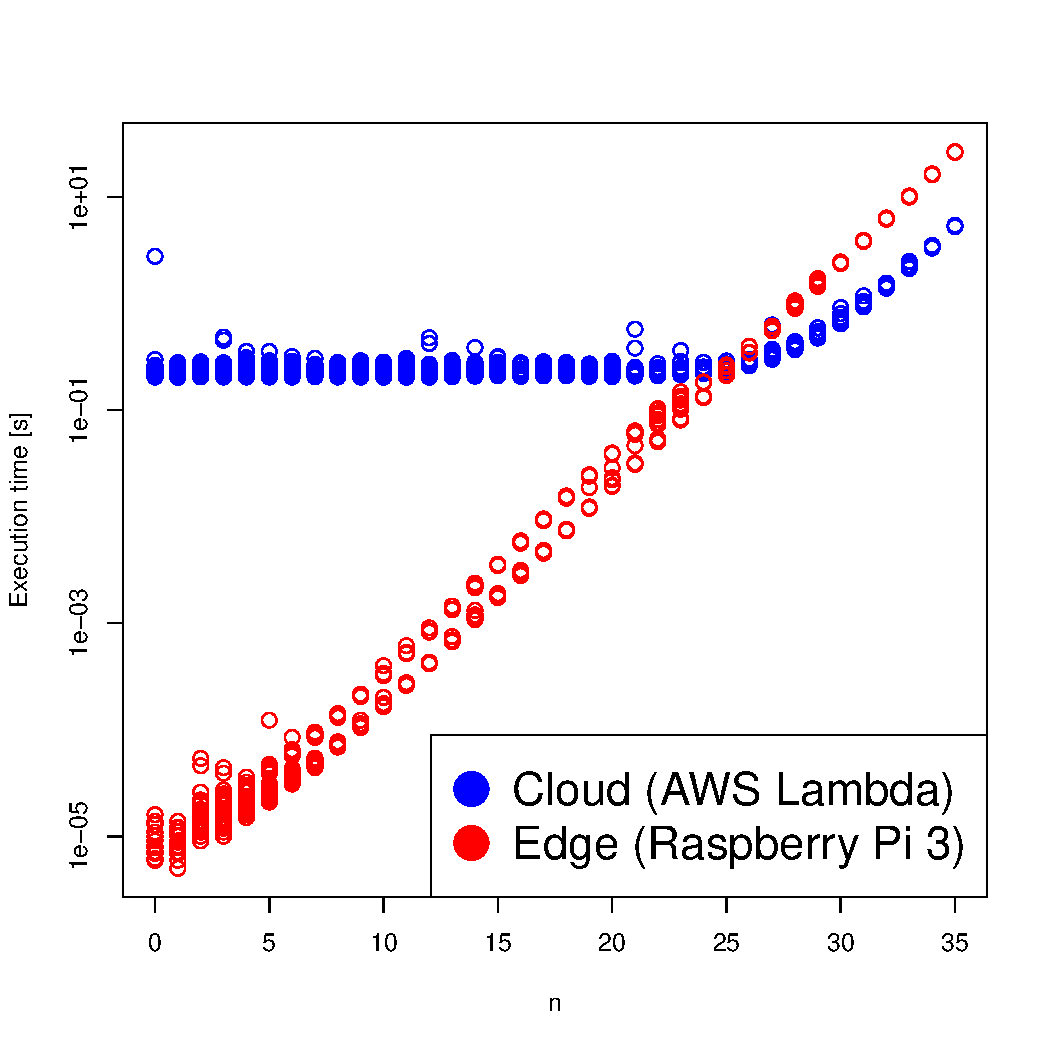
\includegraphics[width=10cm]{figures/Rplots}
% \caption[Experimental results]{Execution time of solving a computationally expensive problem either on the cloud or on the edge device itself. $n$ denotes the computed index in the Fibonachi sequence.}
% \label{fig:experiment}
% \end{center}

% \end{figure}
% \section{Minimizing Edge Computing Latency}\label{sec:experiment}
% As discussed in \autoref{sec:pros-and-cons} can edge computing be used to decrease latency compared to using cloud solutions.
% However, edge nodes have less resources available than public clouds.
% Therefore it is important to take into account how computationally expensive a task is before deciding where to schedule the execution of the task~\cite{gorlatova_characterizing_2018}.
% Gorlatova et al.~\cite{gorlatova_characterizing_2018} presented an algorithm to address this problem.
% This algorithm requires an accurate estimation of how expensive the computation is in order to optimally schedule the task.
% Such estimation is not always possible, therefore we propose a novel method which ensures minimal latency for such scheduling problem.
% Simultaneously scheduling the same task at both the edge and cloud allows opportunistic usage of the result resource which finished first.

% In order to test this approach was an experiment conducted, which executes increasingly computationally expensive tasks both at the edge and cloud.
% The task was implemented as a serverless function in AWS Lambda, deployed to a Raspberry Pi 3 running AWS Greengrass Core and the AWS public cloud as our edge and cloud solution respectively.
% As computation task was a recursive implementation of the Fibonacci sequence used, which complexity grows exponentially.
% \autoref{fig:experiment} presents the results of the experiment.

% The measured results reflect the expected exponential growth of the execution time both on the edge and in the cloud.
% For lower values of $n$ is the edge faster as the overhead of invoking cloud functions dominates the duration of the computation on the cloud.
% However, with values of $n$ exceeding $25$ starts the cloud to outperform the edge node, as the processors in the cloud are faster than the ones of the Raspberry Pi.

%============================================================
\section{Discussion \& Conclusion}\label{sec:discussion-conclusion}
As described in the previous section, several public cloud providers now offer edge computing environments that allow edge devices (owned by the end-users) to integrate with their cloud solutions.
Edge computing offers advantages over cloud computing, including decreased latency, lower bandwidth usage and offline operation~\cite{shi_edge_2016}.
Some of these edge computing solutions offered by public cloud providers also include support for executing serverless functions similar to these deployed on their serverless cloud platform.
Employing the serverless paradigm on edge computing abstracts away the hardware details, thus relieving the developer from the burden of supporting individual hardware configurations on different edge nodes~\cite{nastic_serverless_2017}.

This paper compares two serverless edge computing solutions offered by public cloud providers, namely AWS Greengrass~\cite{amazon_aws_nodate} and Microsoft Azure IoT Edge~\cite{microsoft_iot_2018}, to a self proposed combination of IBM Cloud Functions~\cite{ibm_cloud_2018} with Apache OpenWhisk~\cite{the_apache_software_foundation_apache_nodate}.
Although IBM Cloud Functions does not provide a serverless edge solution, their runtime is based on OpenWhisk, which is open-source and can thus be deployed on edge devices.
Both AWS Greengrass and Azure IoT Edge are generally available, however it is clear that both platforms are still under heavy development, Azure Functions is even still in ``public preview''.
All solutions differ in the set of programming languages they support, however many similarities exist, in particular Java and Javascript supported by all of them.
The solutions from the public cloud providers both offer a device management tool, which is an great advantage over the combination of IBM Cloud Functions with Apache OpenWhisk.
The device management tools offer a platform to which all edge devices connect.
This platform simplifies managing vasts amounts of edge nodes by offering various features, including health monitoring of all devices, updating firmware and software remotely for multiple devices and aggregating logs.

% Our proposed method on lowering latency for tasks with widely varying computational costs is trivially not perfectly resource efficient.
% As the computation will always be partially executed twice.
% We observer that the overhead of the cloud function is nearly constant, hence the edge device can abort its computation when the faster processor speeds of the cloud made up for the overhead to move the computation to the cloud.


The adoption of serverless edge computing by two major players in the public cloud computing industry is a strong signal that these technologies are starting to gain usage in practical solutions.
However, we faced difficulties finding scientific research to support the advantages and possible use cases of such technology.
Hence more research is needed on the integration of the serverless paradigm onto edge devices.
The ongoing developments made by AWS and Azure in this field are a potential source of knowledge, experience and inspiration for future academic research.

%============================================================
\newpage
\bibliographystyle{plain}
\bibliography{edge-computing}

\end{document}
